%%%%%%%%%%%%%%%%%%%%%%%%%%%%%%%%%%%%%%%%%
% baposter Landscape Poster
% LaTeX Template
% Version 1.0 (11/06/13)
%
% baposter Class Created by:
% Brian Amberg (baposter@brian-amberg.de)
%
% This template has been downloaded from:
% http://www.LaTeXTemplates.com
%
% License:
% CC BY-NC-SA 3.0 (http://creativecommons.org/licenses/by-nc-sa/3.0/)
%
%%%%%%%%%%%%%%%%%%%%%%%%%%%%%%%%%%%%%%%%%

%----------------------------------------------------------------------------------------
%	PACKAGES AND OTHER DOCUMENT CONFIGURATIONS
%----------------------------------------------------------------------------------------

\documentclass[landscape,a0paper,fontscale=0.285]{baposter} % Adjust the font scale/size here

\usepackage{graphicx} % Required for including images
\graphicspath{{figures/}} % Directory in which figures are stored

\usepackage{amsmath} % For typesetting math
\usepackage{amssymb} % Adds new symbols to be used in math mode

\usepackage{booktabs} % Top and bottom rules for tables
\usepackage{enumitem} % Used to reduce itemize/enumerate spacing
\usepackage{palatino} % Use the Palatino font
\usepackage[font=small,labelfont=bf]{caption} % Required for specifying captions to tables and figures

\usepackage{multicol} % Required for multiple columns
\setlength{\columnsep}{1.5em} % Slightly increase the space between columns
\setlength{\columnseprule}{0mm} % No horizontal rule between columns

\usepackage{tikz} % Required for flow chart
\usetikzlibrary{shapes,arrows} % Tikz libraries required for the flow chart in the template

\usepackage{relsize}

\newcommand{\compresslist}{ % Define a command to reduce spacing within itemize/enumerate environments, this is used right after \begin{itemize} or \begin{enumerate}
\setlength{\itemsep}{1pt}
\setlength{\parskip}{0pt}
\setlength{\parsep}{0pt}
}

\definecolor{lightblue}{rgb}{0.145,0.6666,1} % Defines the color used for content box headers

\begin{document}

\begin{poster}
{
headerborder=closed, % Adds a border around the header of content boxes
colspacing=1em, % Column spacing
bgColorOne=white, % Background color for the gradient on the left side of the poster
bgColorTwo=white, % Background color for the gradient on the right side of the poster
borderColor=lightblue, % Border color
headerColorOne=black, % Background color for the header in the content boxes (left side)
headerColorTwo=lightblue, % Background color for the header in the content boxes (right side)
headerFontColor=white, % Text color for the header text in the content boxes
boxColorOne=white, % Background color of the content boxes
textborder=roundedleft, % Format of the border around content boxes, can be: none, bars, coils, triangles, rectangle, rounded, roundedsmall, roundedright or faded
eyecatcher=true, % Set to false for ignoring the left logo in the title and move the title left
headerheight=0.132\textheight, % Height of the header
headershape=roundedright, % Specify the rounded corner in the content box headers, can be: rectangle, small-rounded, roundedright, roundedleft or rounded
headerfont=\Large\bf\textsc, % Large, bold and sans serif font in the headers of content boxes
%textfont={\setlength{\parindent}{1.5em}}, % Uncomment for paragraph indentation
linewidth=2pt % Width of the border lines around content boxes
}
%----------------------------------------------------------------------------------------
%	TITLE SECTION 
%----------------------------------------------------------------------------------------
%
{
\includegraphics[height=3em]{anr}} % First university/lab logo on the left
{\bf\textsc{Testing the upper-mantle seismic signature of plume- \\ \vspace{0.05em} lithosphere interaction in the northern East-African Rift}\vspace{0.2em}} % Poster title
{\textsc{ Chiara Civiero, \textbf{John Armitage}, Sakia Goes, James Hammond}  \\ cciviero@cp.dias.ie, armitage@ipgp.fr, saskia.goes@imperial.ac.uk, j.hammond@ucl.ac.uk\vspace{0.3em}} % Author names and institution
{
\includegraphics[height=5em]{LogoIPGP}} % Second university/lab logo on the right


%----------------------------------------------------------------------------------------
%	Introduction
%----------------------------------------------------------------------------------------

\headerbox{Introduction}{name=introduction,column=0,row=0}{

Below the northern East African Rift two low seismic velocity zones are imaged. \textbf{Are these due to the rising thermal anomalies?} We will explore this hypothesis by generating synthetic tomography from models of the convective destabilization of hot mantle.

\begin{center}
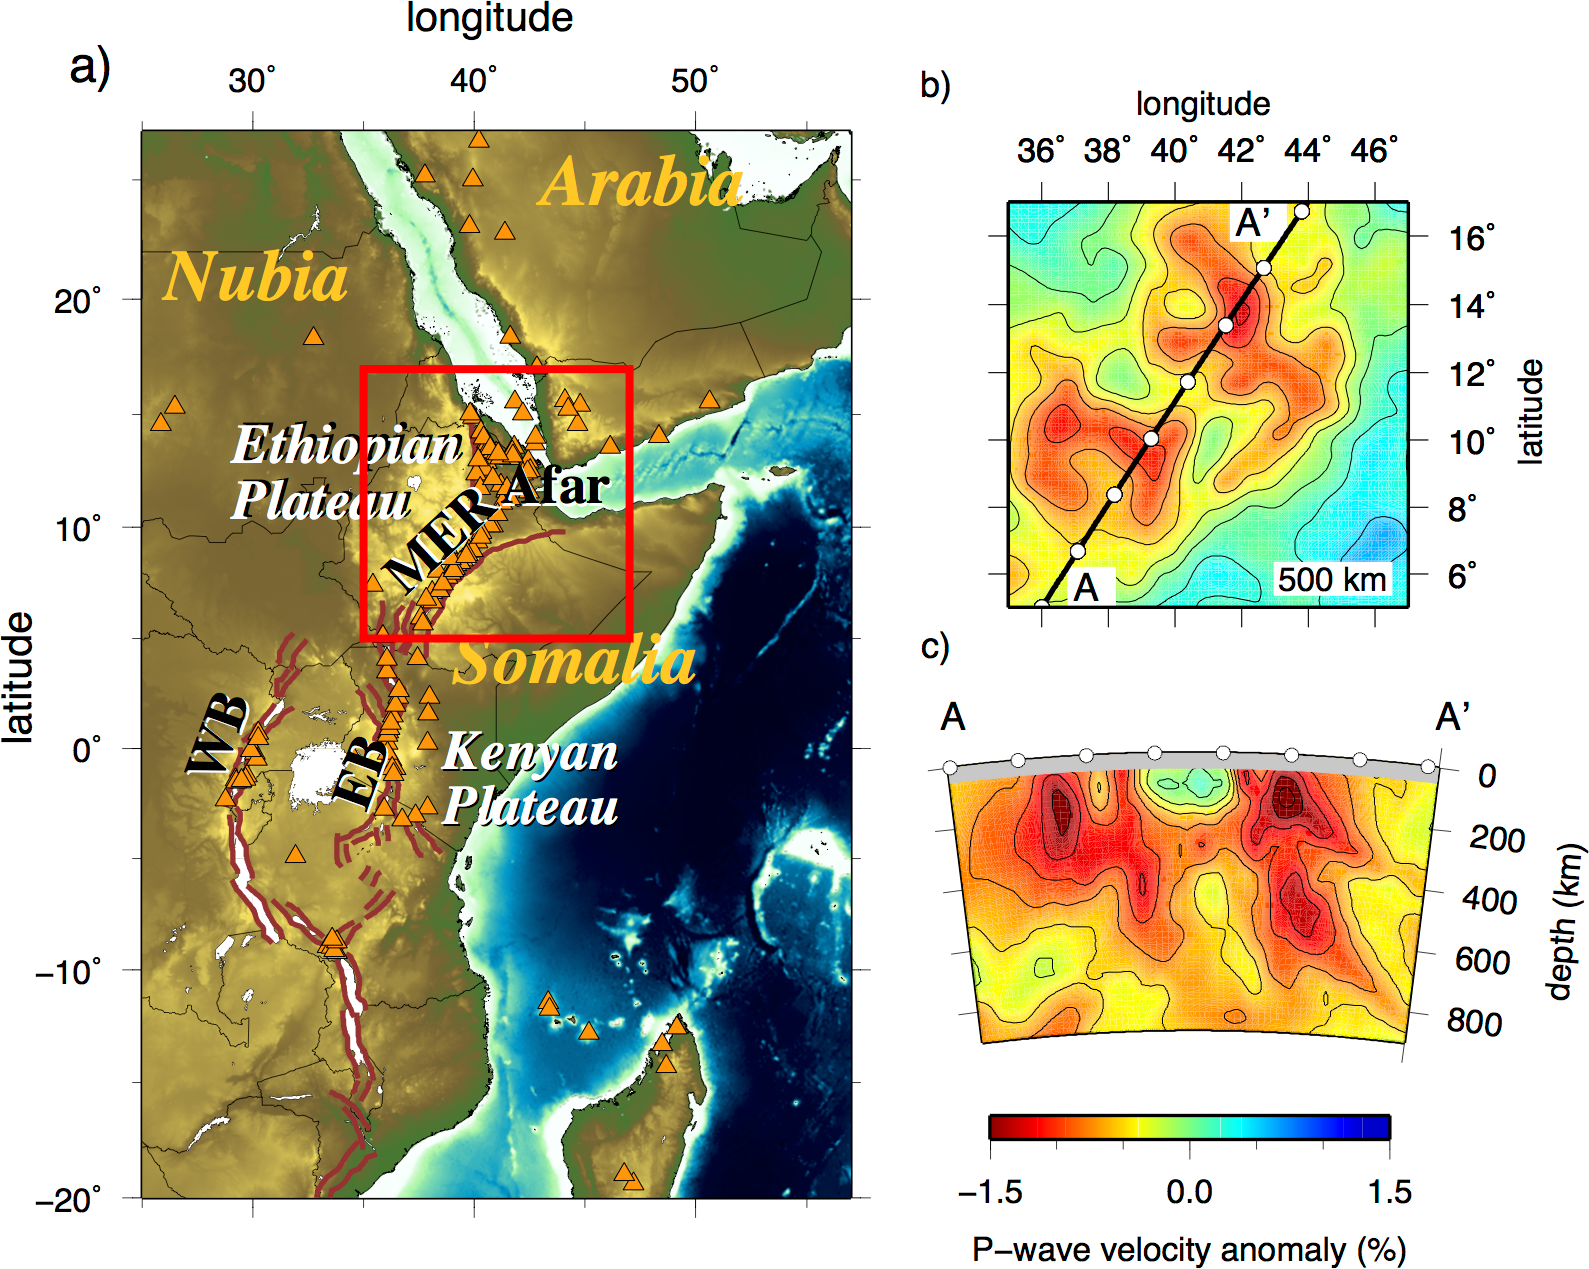
\includegraphics[width=0.8\linewidth]{fig01}
\captionof{figure}{The northern East African Rift and slices from the P-wave tomographic model NEAR-P15 \cite{civiero-etal-2015}.}
\end{center}

\vspace{0.3em} % When there are two boxes, some whitespace may need to be added if the one on the right has more content
}

%----------------------------------------------------------------------------------------
%	Methods
%----------------------------------------------------------------------------------------

\headerbox{Geodynamic to Seismic}{name=methods,column=3,row=0,bottomaligned=introduction}{

\smaller

Both RB convection and RT instabilities are generated by solving for Stokes flow in a Cartesian box using the code Stag3D \cite{tackley-1998}. Temperature and pressure are converted to mineral phases assuming a pyrolite composition for the mantle and harzbugite for the lithosphere. This gives the anharmonic seismic velocity. This is corrected for attenuation using the $Q_{g}$ model \cite{goes-etal-2012}.

\begin{center}
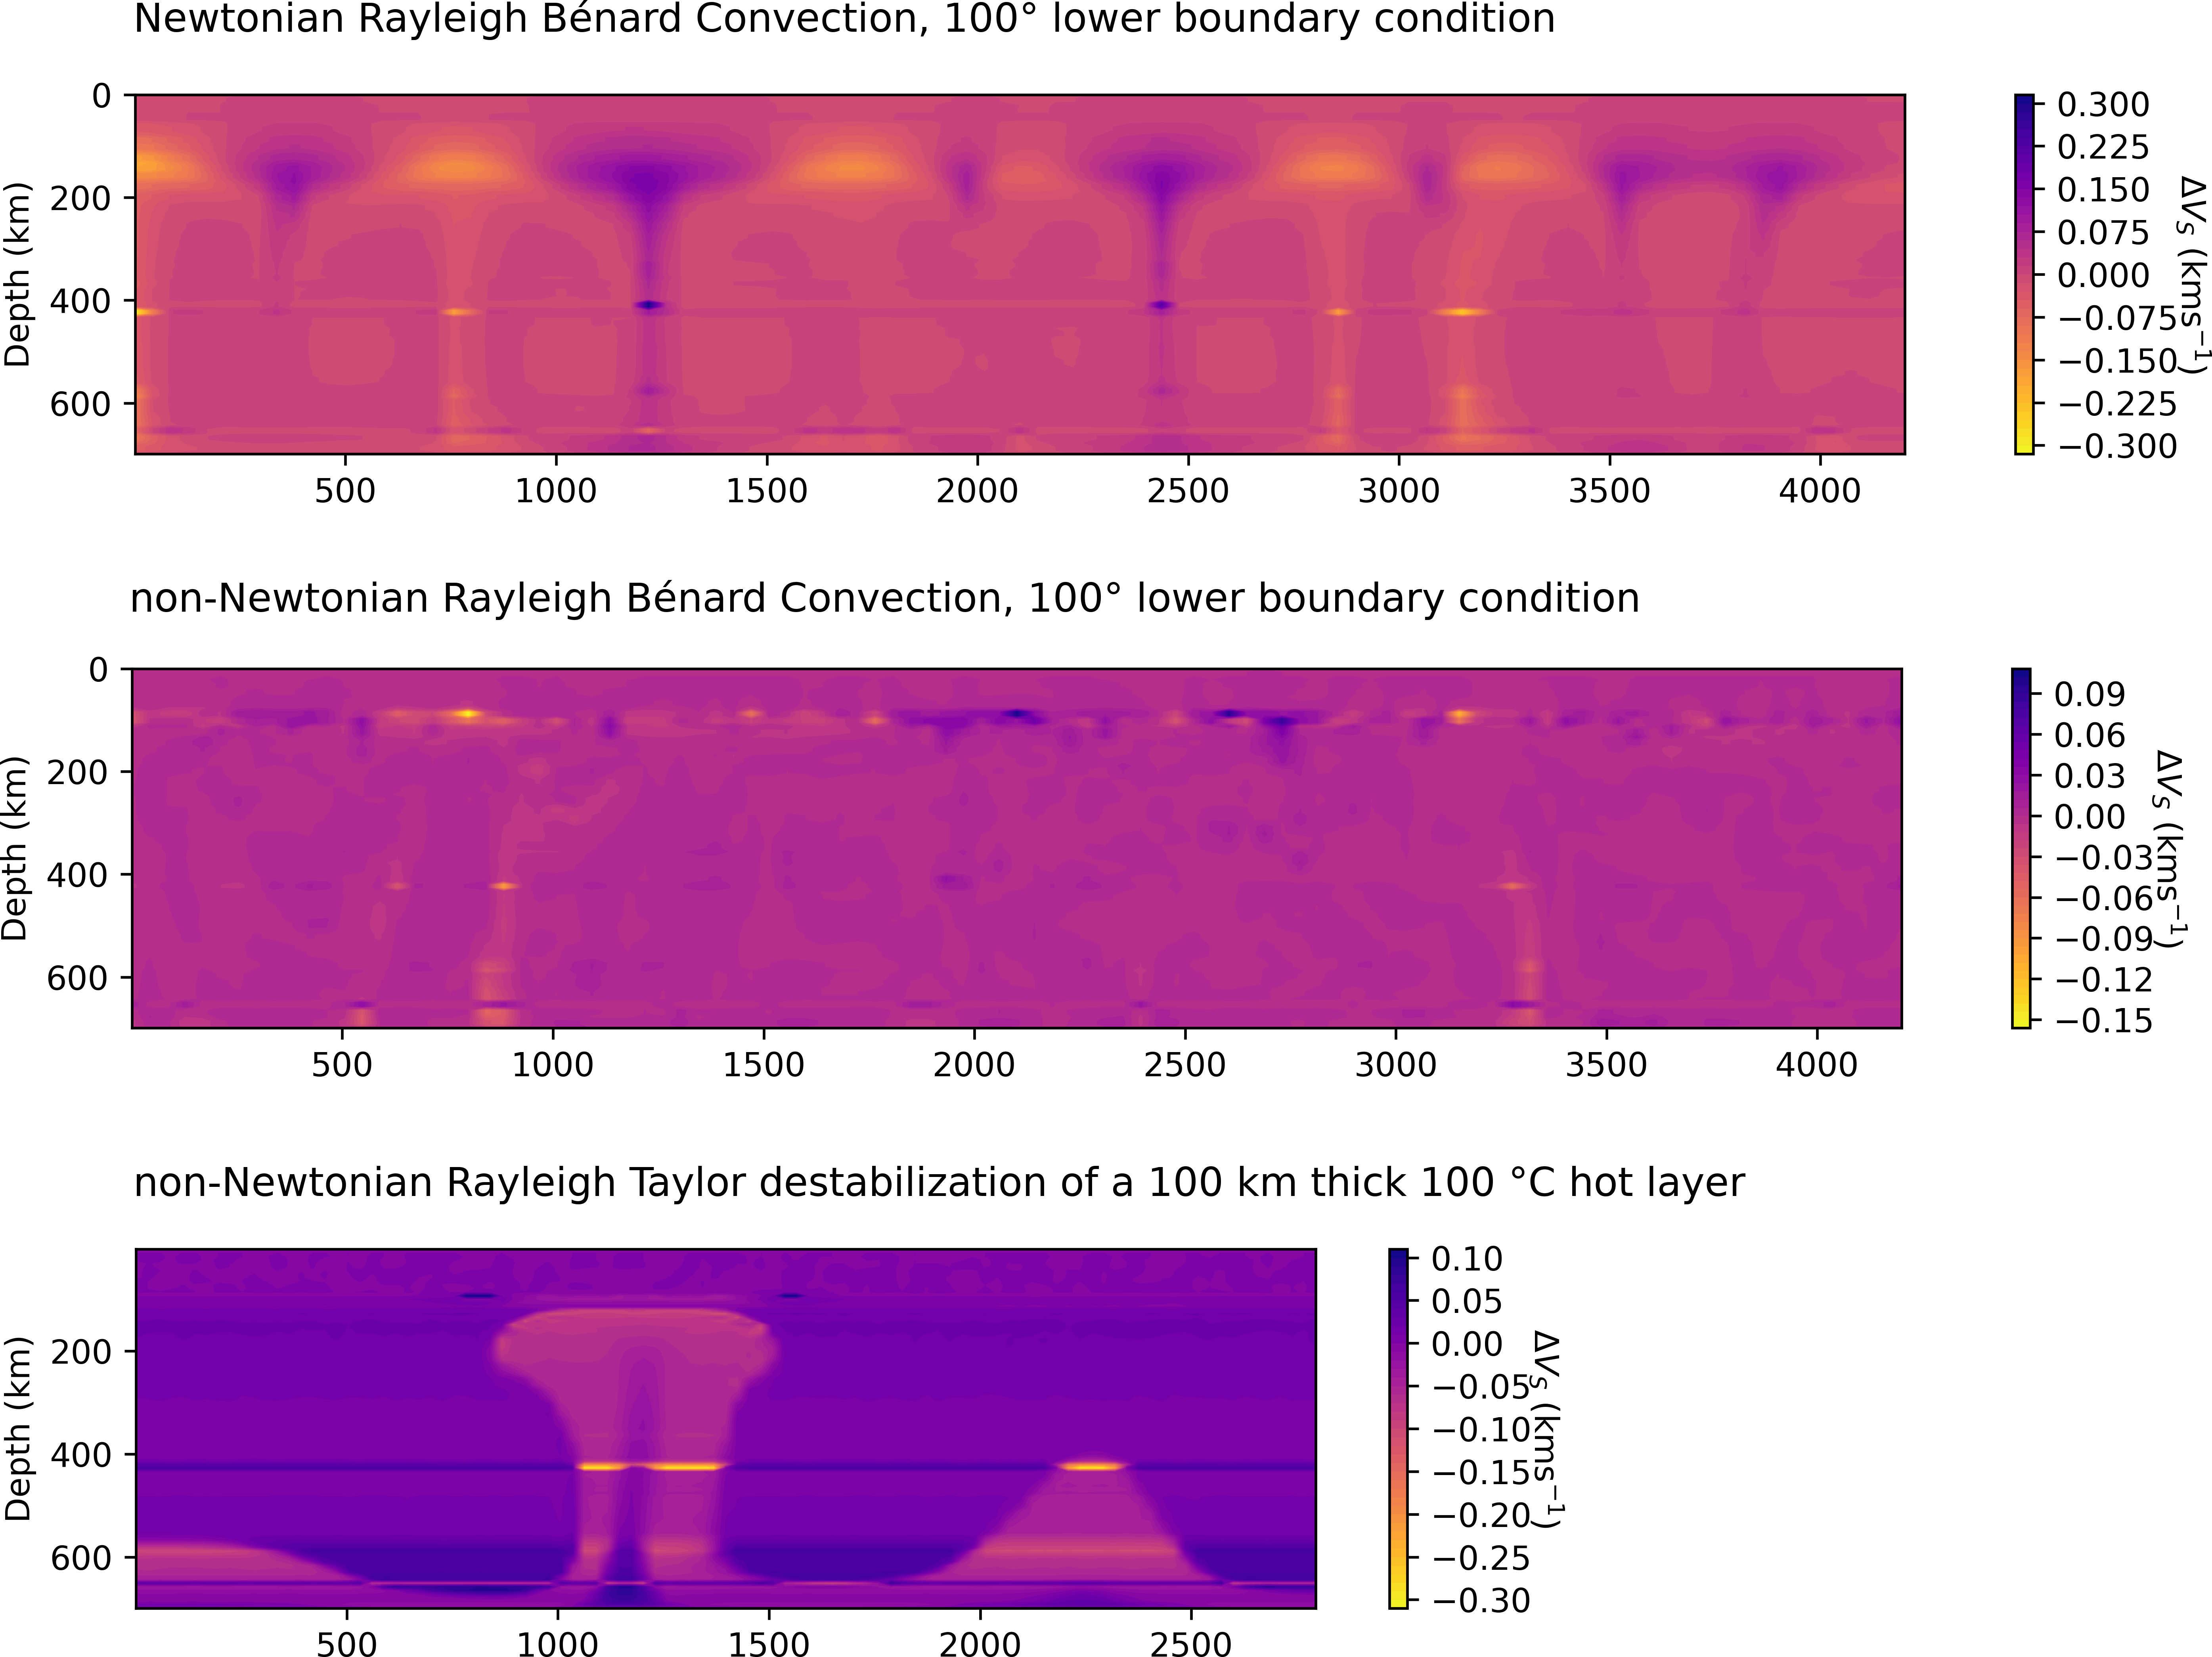
\includegraphics[width=0.8\linewidth]{velocities}
\captionof{figure}{2D slices of the S-wave velocity anomalies for RB convection with a Newtonian rheology, a non-Newtonian rheology, and RT destabilization of a hot layer. Anomalies are relative to the horizontal average.}
\end{center}
}

%----------------------------------------------------------------------------------------
%	RESULTS 1
%----------------------------------------------------------------------------------------

\headerbox{Rayleigh B{\'e}nard or Rayleigh Taylor?}{name=results,column=1,span=2,row=0}{

For Raleigh B{\'e}nard (RB) convection the wavelength between plumes, $\lambda$, varies as $Ra^{1/6}$ \cite{galsa-2007}. For Raleigh Taylor (RT) destabilization of a hot layer, $\lambda$, varies as a linear function of the model height \cite{schmeling-1987}. The observed spacing of the two low seismic velocity structures is $\sim700$\,km (Figure 1). We find that for RB convection this implies a $10^6 < Ra < 10^7$ (e.g. Figure 3). For RT destabilization this is consistent with a model aspect ratio of 3x3x1 (Figure 4a). Plume development for RT destabilization is also time dependent with early, mid and late stage plumes (ES, MS, and LS, Figure 4b). 


\begin{minipage}{.48\linewidth}
	\begin{center}
		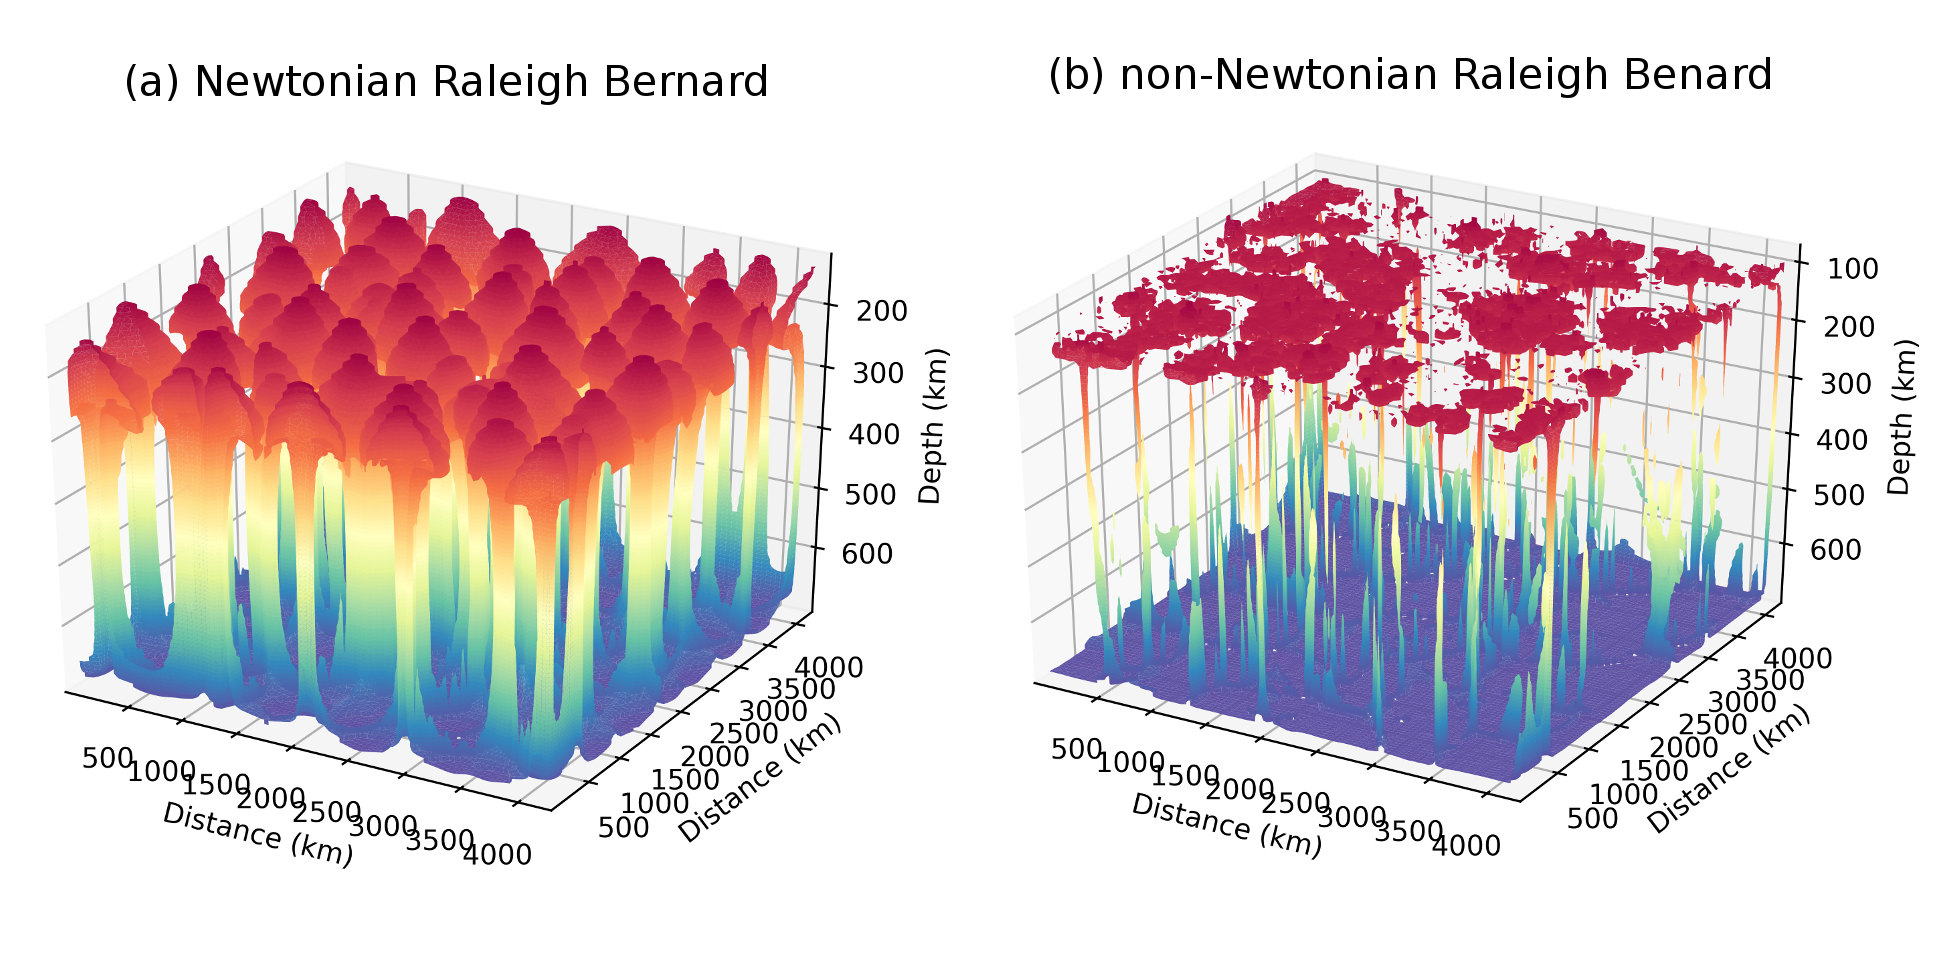
\includegraphics[width=0.95\linewidth]{comparison}
		\captionof{figure}{RB convection for (a) Newtonian and (b) non-Newtonian creep with a $100\rm\,^{\circ}C$ hot lower boundary condition.}
	\end{center}
\end{minipage}
\begin{minipage}{.04\linewidth}
\end{minipage}
\begin{minipage}{.48\linewidth}
	\begin{center}
	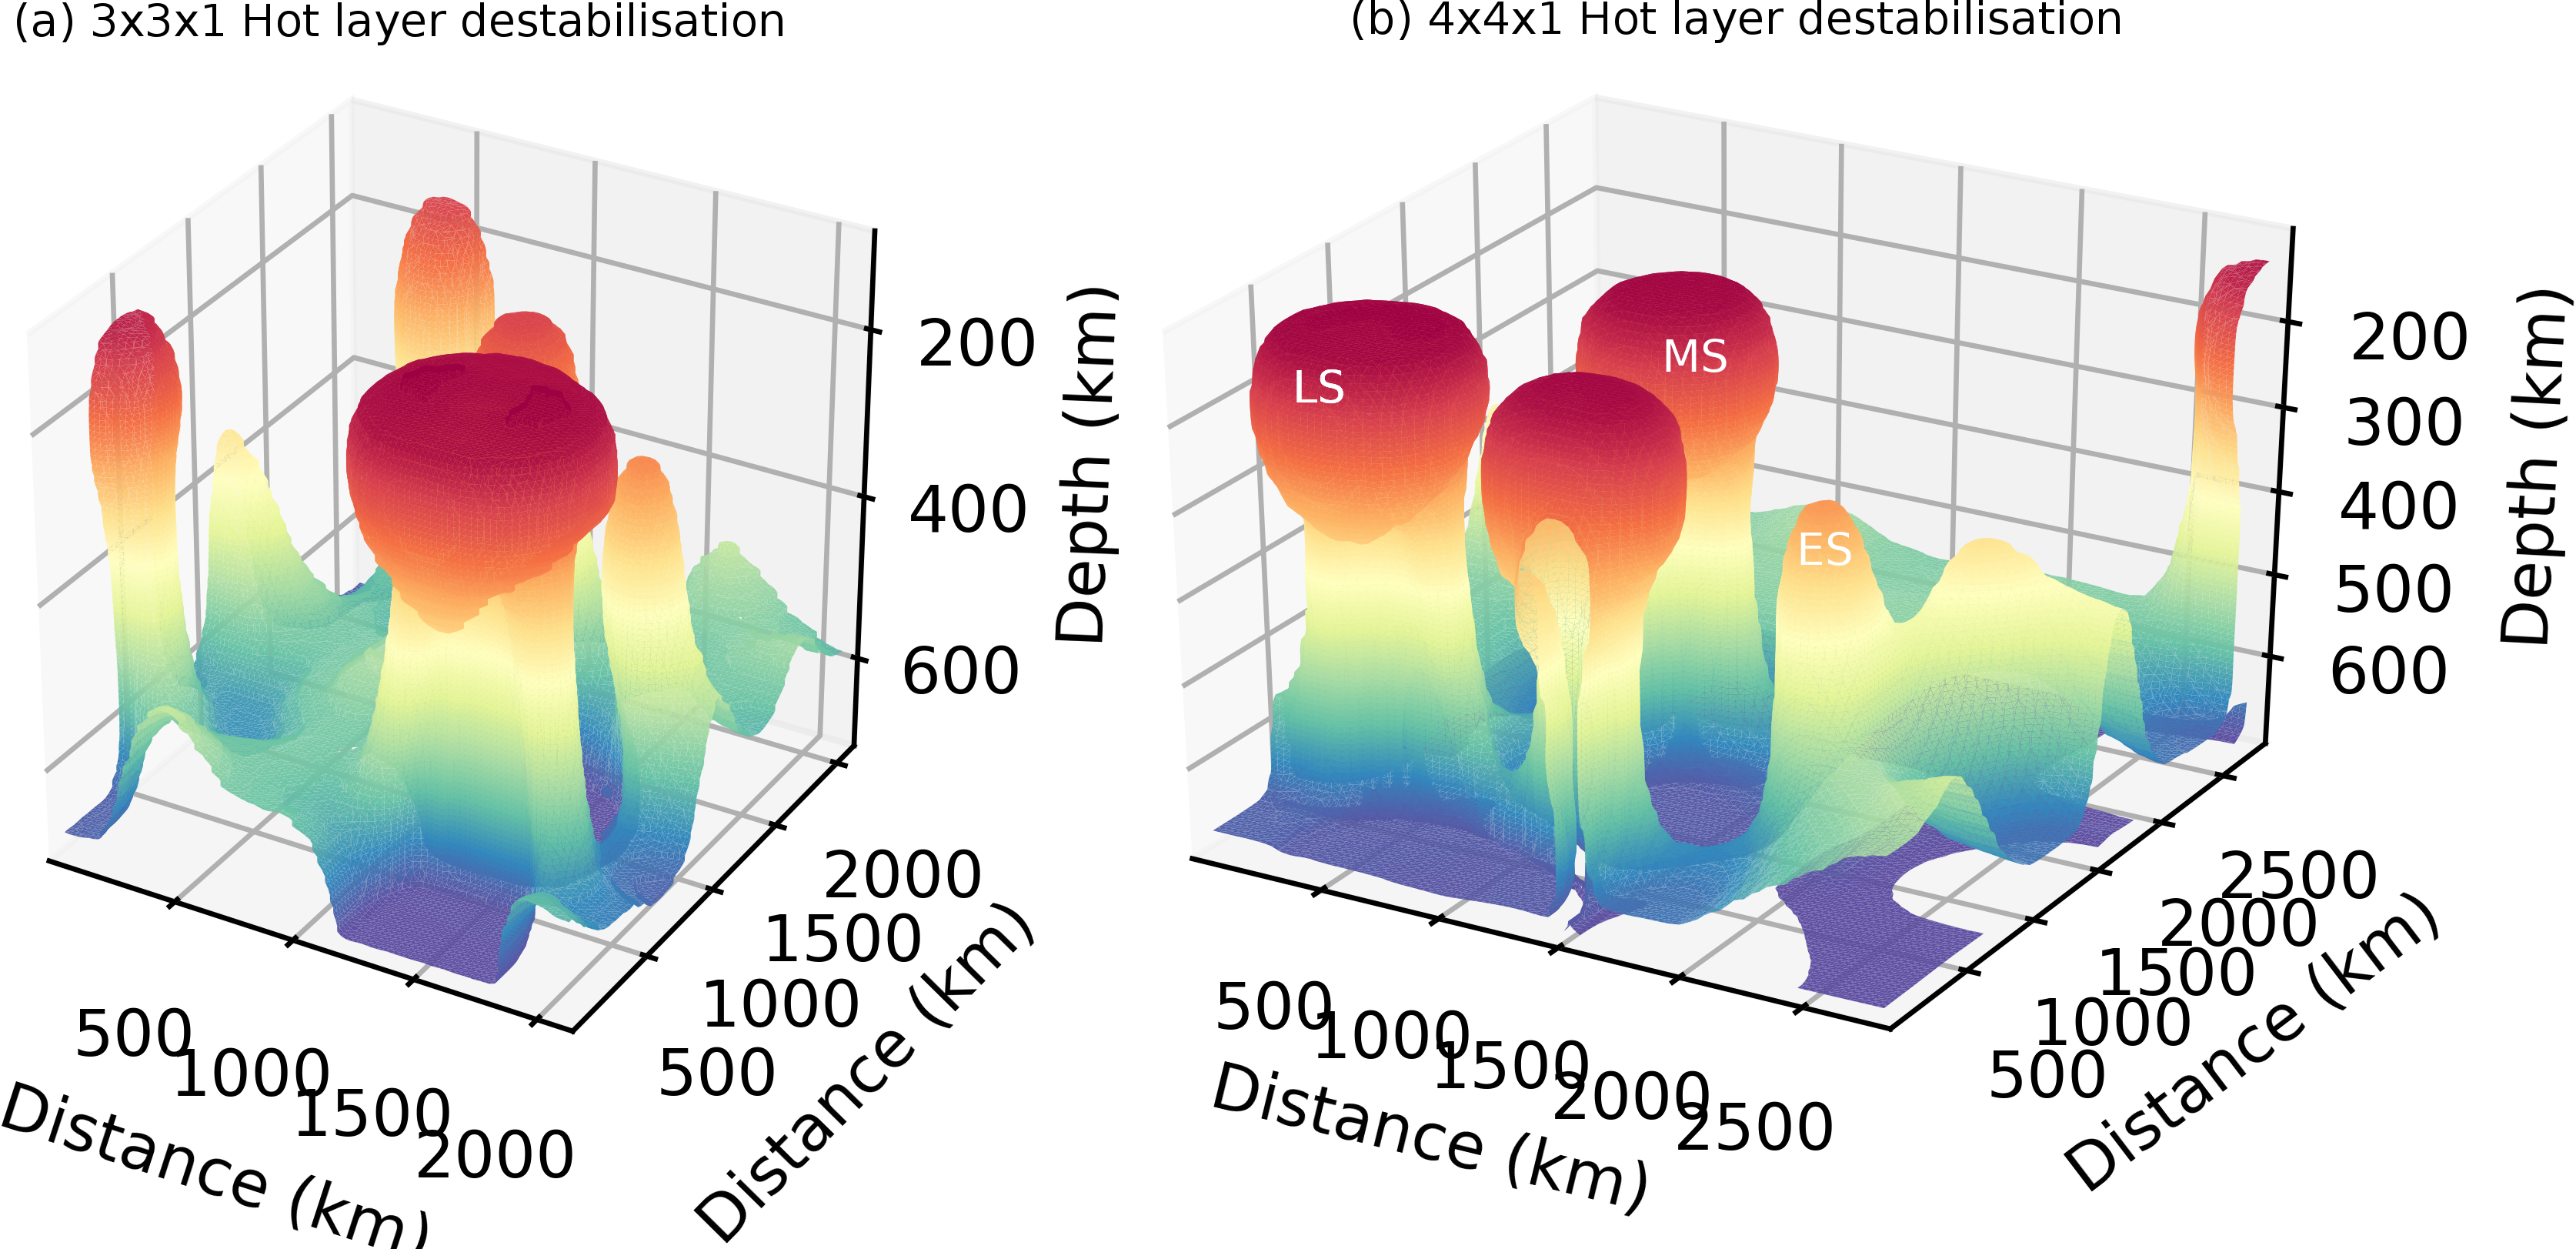
\includegraphics[width=0.95\linewidth]{comparison-3x4-lables.png}
	\captionof{figure}{RT destabilization for a $100\rm\,^{\circ}C$ 100\,km thick hot layer. Aspect ratios of (a) 3x3x1 and (b) 4x4x1. ES - Eary stage; MS Mid-stage; and LS Late stage plumes.}
	\end{center}
\end{minipage}

}

%----------------------------------------------------------------------------------------
%	REFERENCES
%----------------------------------------------------------------------------------------

\headerbox{References}{name=references,column=0,below=introduction}{

\renewcommand{\section}[2]{\vskip 0.05em} % Get rid of the default "References" section title
\nocite{*} % Insert publications even if they are not cited in the poster
\small{ % Reduce the font size in this block
\bibliographystyle{unsrt}
\bibliography{sample.bib} % Use sample.bib as the bibliography file
}}

%----------------------------------------------------------------------------------------
%	ACKNOWLEDGEMENTS
%----------------------------------------------------------------------------------------

\headerbox{Acknowledgements}{name=acknowledgements,column=0,below=references, above=bottom}{

This work was funded by a Agence Nationale de la Recherche grant to John Armtiage and a Janet Watson Fellowship awarded to Chiara Civiero.
} 

%----------------------------------------------------------------------------------------
%	Conclusions
%----------------------------------------------------------------------------------------

\headerbox{Conclusions}{name=conclusions,column=3,span=1,aligned=references,below=methods,above=bottom}{ % This block is as tall as the references block

\begin{enumerate}
    \item The thermal anomalies below Afar and the Main Ethiopian Rift are the form of rising plumes.
    \item Seismic tomography from the dense array of seismometers in the northern East African Rift is consistent with the Rayleigh Taylor-like destabilization of a hot layer of mantle at or below the 660\,km discontinuity.
    \item The plume-like structures are not secondary plumes from a stalled super-plume, but the hot material has its origins in the lower mantle. The hot material subsequently destabilized.
    \item One possible mechanism for such destabilization of ponded material is internal heating, which can give additional buoyancy to thermo-chemical plumes \cite{fourel-etal-2018}.
\end{enumerate}

}


%----------------------------------------------------------------------------------------
%	Results 2
%----------------------------------------------------------------------------------------

\headerbox{Synthetic Tomography: Rayleigh Taylor wins}{name=results2,column=1,span=2,row=0,below=results,above=bottom}{

It was found that while the spacing of Newtonian RB plumes was consistent with observations, the anomalies are too weak. The RT destabilization of a hot layer however gives a pattern of seismic anomalies that matches the observations (Figure 5). The RT destabilization of a $200\rm\,^{\circ}C$ hot layer perhaps has a magnitude reduction in seismic velocity that is in closer agreement to the observed anomalies (Figure 6).


%------------------------------------------------

\begin{minipage}{.48\linewidth}
	\begin{center}
		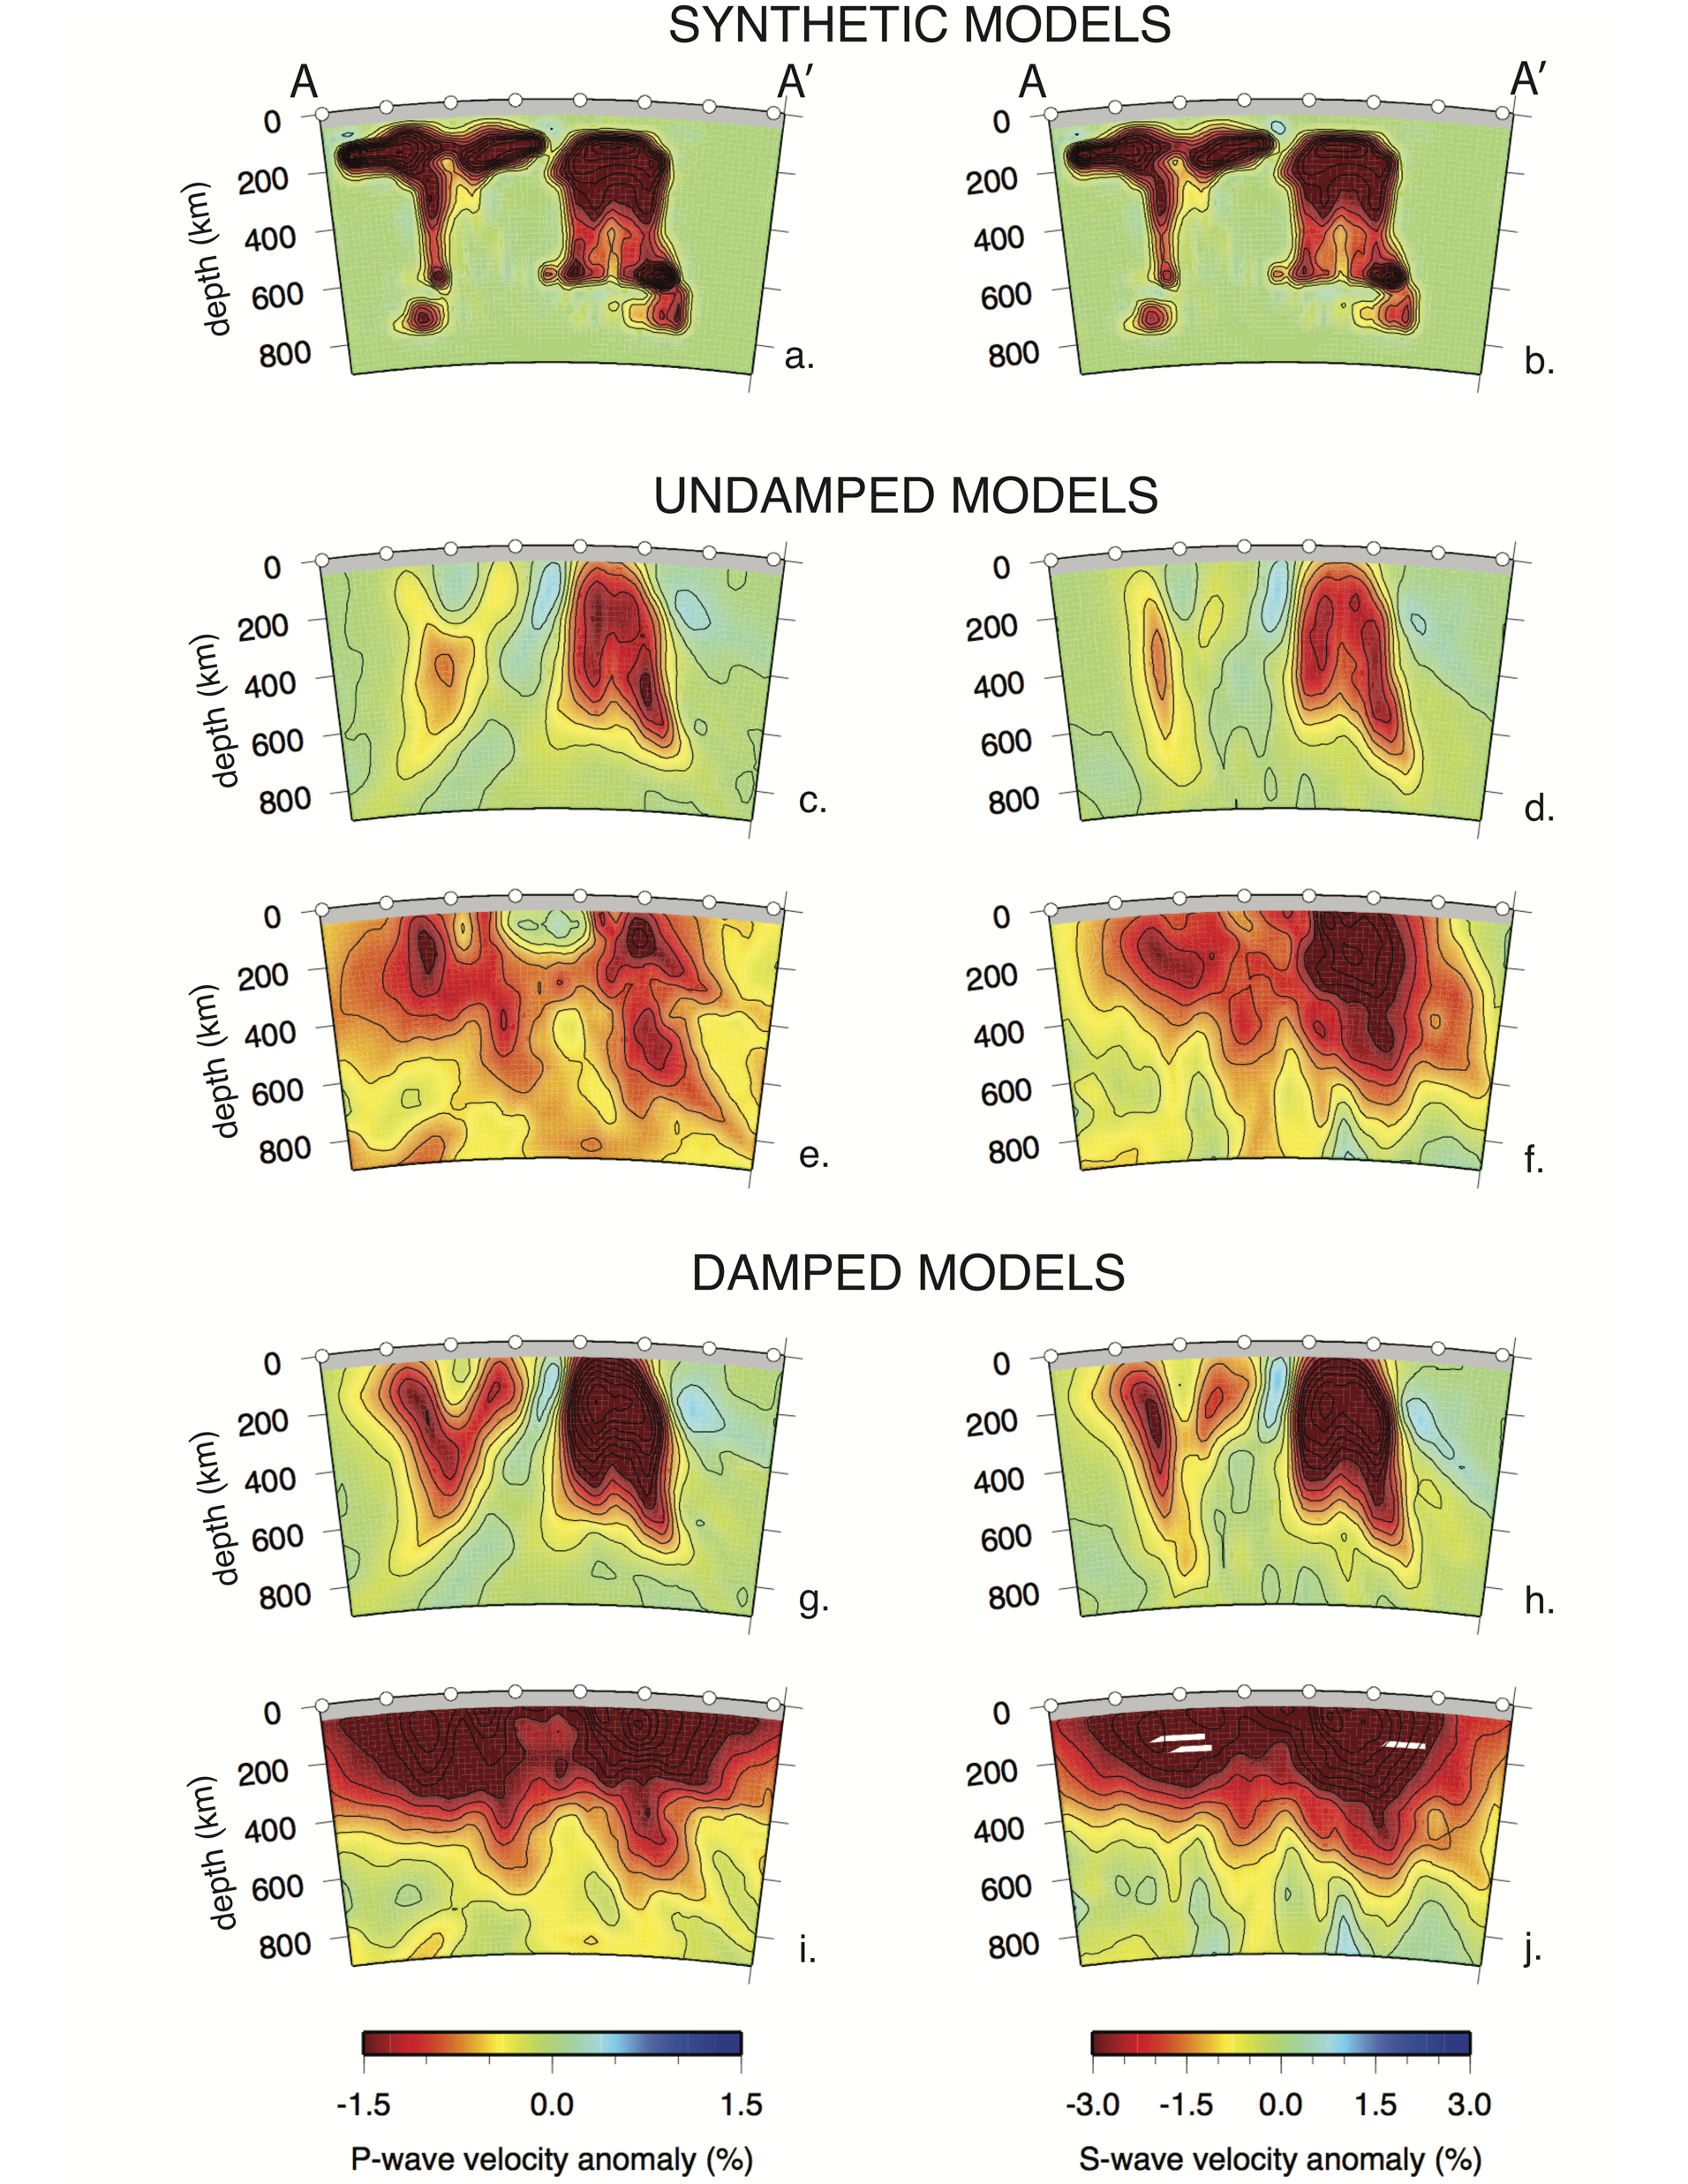
\includegraphics[width=0.95\linewidth]{fig07}
		\captionof{figure}{Conversion of RT destabilization (Figure 4a) to synthetic seismic tomography using the same parameters as for the observed tomography (Figure 1).}
	\end{center}
\end{minipage}
\begin{minipage}{.04\linewidth}
\end{minipage}
\begin{minipage}{.48\linewidth}
	\begin{center}
		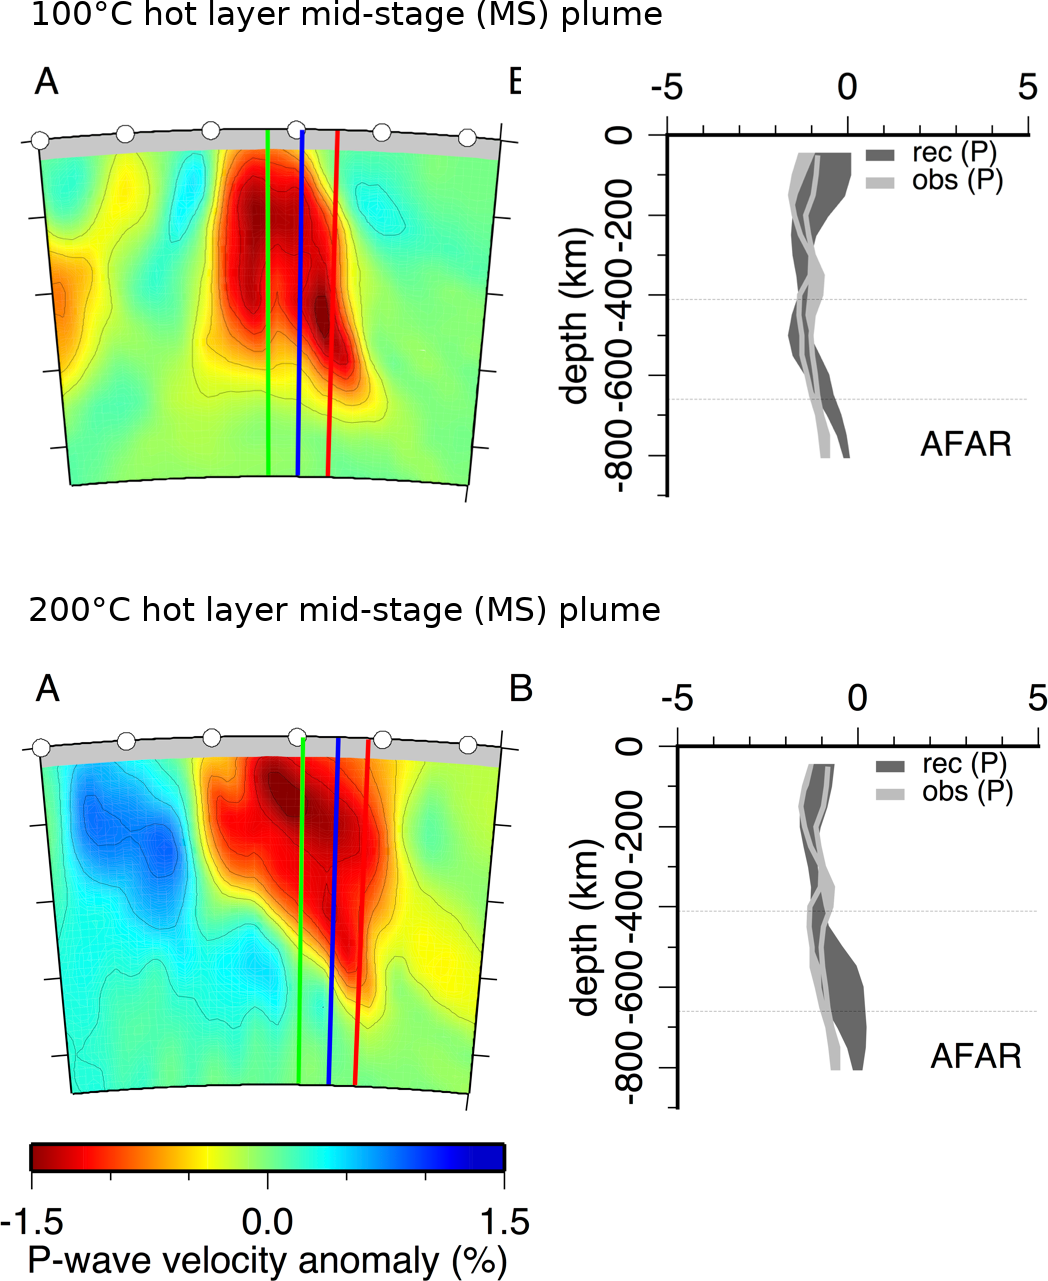
\includegraphics[width=.6\linewidth]{synth-comp}
		\captionof{figure}{Comparison of the observed magnitude of $V_{P}$ below Afar with two mid-stage plumes (MS in Figure 4b) with different hot layer temperatures.}
	\end{center}
\end{minipage}
}


%----------------------------------------------------------------------------------------

\end{poster}

\end{document}